\documentclass[11pt,a4paper]{article}
\usepackage[latin5]{inputenc}
\usepackage[english]{babel}
\usepackage{amsmath}
\usepackage{amsfonts}
\usepackage{amssymb}
\usepackage{graphicx,subfig}
\usepackage{placeins}
\usepackage{gensymb}

\author{Alexander Attinger, Yannic Kilcher}
\title{Report Sheet 1, Advanced Part}

\begin{document}
\maketitle


\section{Image Retrieval}
\paragraph{Histograms}
Histograms can be very characteristic for a particular kind of image. This property can be used for image retrieval and a measure of image similarity, i.e. two images are considered similar, if their histograms are similar. Using histograms as a basis of similarity measures is probably very sensitive to change in lightning conditions (i.e. same scene, different time of the day). Also, histograms are context insensitive, i.e. shapes are not taken into account.
\begin{table}
\centering

\begin{tabular}{ |c | r | r | r | r | r | r | }
  \hline                        
   &100 & 300 & 400 & 600 & 700 & 800 \\
  chi-squared & 31 & 33 & 53 & 28 & 29 & 29 \\
  correlation & 38 & 18 & 29 & 12 & 33 & 24 \\
  Bhattaryya & 42 & 28 & 10 & 14 & 21 & 27 \\
  \hline  
  
\end{tabular}
\caption{Comparing different distance measures. Number of images that need to be taken into account until all 10 images of a set are retrieved.}
\label{table:1}
\end{table}

\paragraph{Distance Measure}
 A big challenge in image retrieval using histograms is the method used for comparing the histograms. We compared three different distance measured: Chi-Squared, Correlation and Bhattacharyya. The effect of the distance measure is quite significant. This can be observed in Figures \ref{fig:1}-\ref{fig:3}. Table \ref{table:1} also shows this effect. It is most pronounced probably for the dinosaur images (400). The Chi squared measure and the Bhattaryya measure both are not very good, but the correlation measure performs very well, the first 10 images retrieved are the ten images of the dataset.
 
 
\paragraph{Histogram equalization}
A technique for enhancing image quality such as constrast is histogram equalization. in an ideal, contrast rich image, the histogram resembles a uniform distribution. From this it is obvious, that image retrieval using histograms from images with equalized histograms should fail. This can be observed in figure \ref{fig:7}. Here, the correlation measure was used to complare the equalized histograms. The reference image was 400, an image of a dinosaur. Only one of the 5 retrieved images acutally shows a dinsoaur, all the others appear quite random. Compare this to table \ref{table:1}, where the first 10 retrieved images were all dinosaurs.

\begin{figure}
\centering
\subfloat[][]{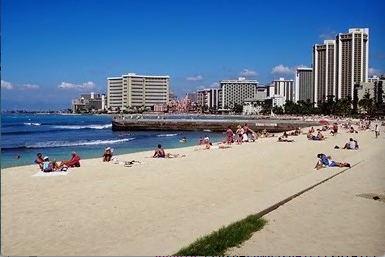
\includegraphics[scale=.4]{img/1001_corr.png}}
\quad
\subfloat[][]{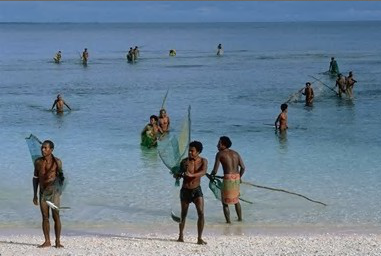
\includegraphics[scale=.4]{img/1002_corr.png}}
\quad
\subfloat[][]{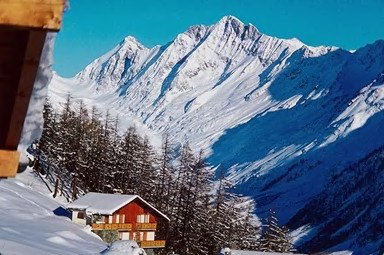
\includegraphics[scale=.4]{img/1003_corr.png}}
\quad
\subfloat[][]{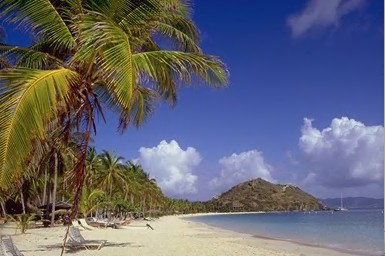
\includegraphics[scale=.4]{img/1004_corr.png}}

\subfloat[][]{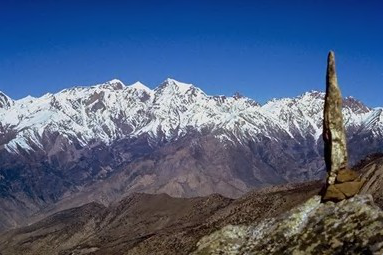
\includegraphics[scale=.4]{img/1005_corr.png}}


\caption{Beach Scene. Using correlation as similarity measure}
\label{fig:1}
\end{figure}

\begin{figure}
\centering
\subfloat[][]{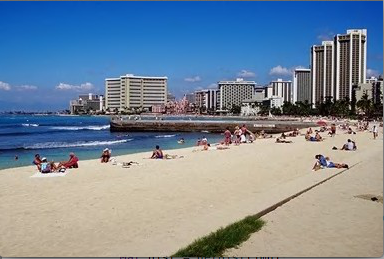
\includegraphics[scale=.4]{img/1001_chi.png}}
\quad
\subfloat[][]{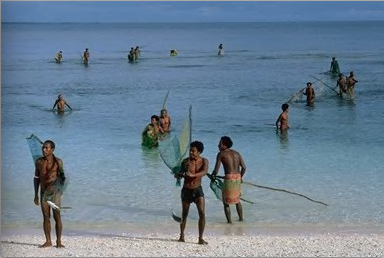
\includegraphics[scale=.4]{img/1002_chi.png}}
\quad
\subfloat[][]{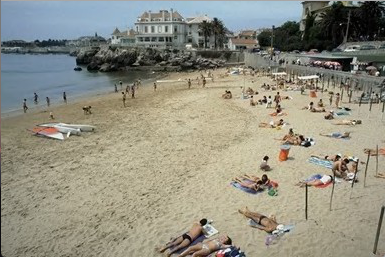
\includegraphics[scale=.4]{img/1003_chi.png}}
\quad
\subfloat[][]{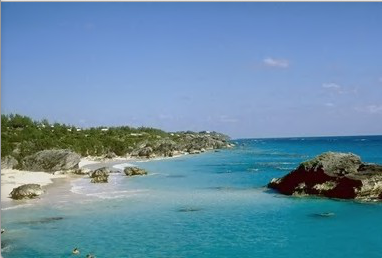
\includegraphics[scale=.4]{img/1004_chi.png}}

\subfloat[][]{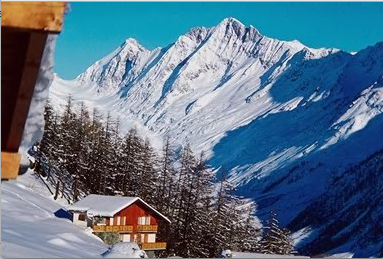
\includegraphics[scale=.4]{img/1005_chi.png}}


\caption{Beach Scene. Using chi-square as similarity measure.}
\label{fig:2}
\end{figure}

\begin{figure}
\centering
\subfloat[][]{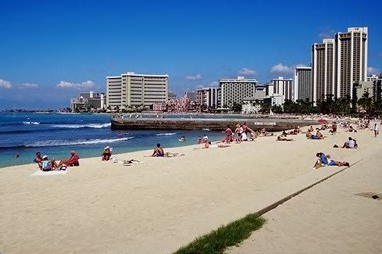
\includegraphics[scale=.4]{img/1001_bhat.png}}
\quad
\subfloat[][]{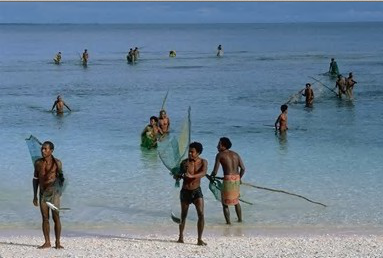
\includegraphics[scale=.4]{img/1002_bhat.png}}
\quad
\subfloat[][]{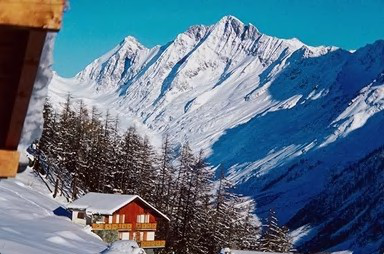
\includegraphics[scale=.4]{img/1003_bhat.png}}
\quad
\subfloat[][]{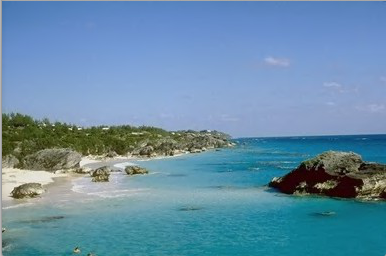
\includegraphics[scale=.4]{img/1004_bhat.png}}

\subfloat[][]{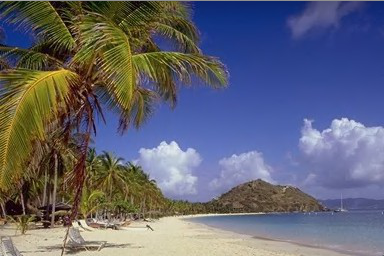
\includegraphics[scale=.4]{img/1005_bhat.png}}


\caption{Beach Scene. Using Bhattacharyya distance as similarity measure.}
\label{fig:3}
\end{figure}


\begin{figure}
\centering
\subfloat[][]{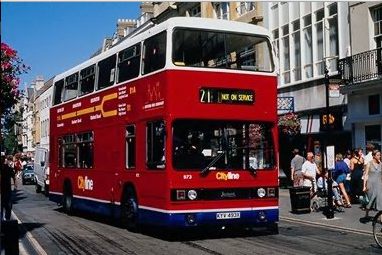
\includegraphics[scale=.4]{img/3001_corr.png}}
\quad
\subfloat[][]{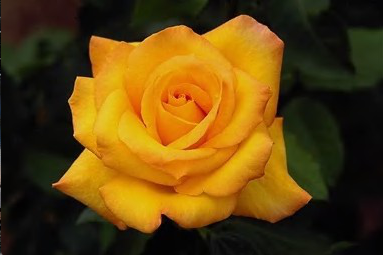
\includegraphics[scale=.4]{img/3002_corr.png}}
\quad
\subfloat[][]{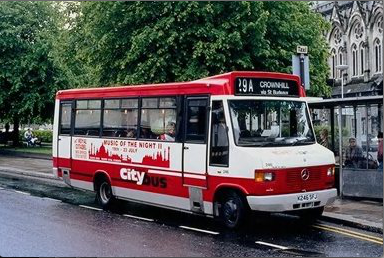
\includegraphics[scale=.4]{img/3003_corr.png}}
\quad
\subfloat[][]{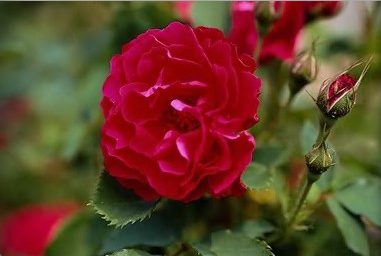
\includegraphics[scale=.4]{img/3004_corr.png}}

\subfloat[][]{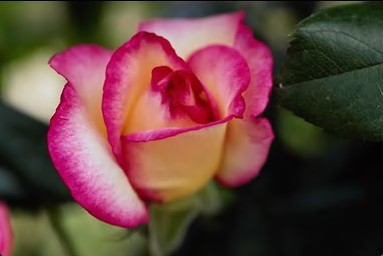
\includegraphics[scale=.4]{img/3005_corr.png}}


\caption{Town Scene. Using correlation as similarity measure}
\label{fig:4}
\end{figure}

\begin{figure}
\centering
\subfloat[][]{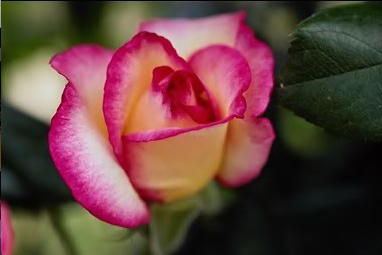
\includegraphics[scale=.4]{img/3001_chi.png}}
\quad
\subfloat[][]{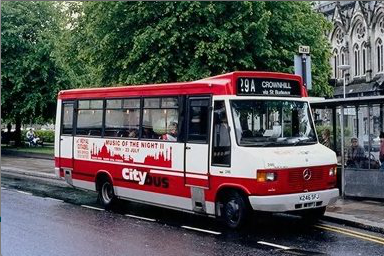
\includegraphics[scale=.4]{img/3002_chi.png}}
\quad
\subfloat[][]{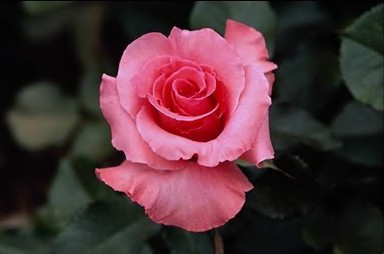
\includegraphics[scale=.4]{img/3003_chi.png}}
\quad
\subfloat[][]{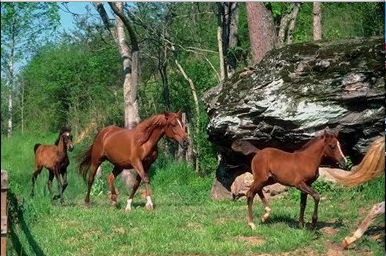
\includegraphics[scale=.4]{img/3004_chi.png}}

\subfloat[][]{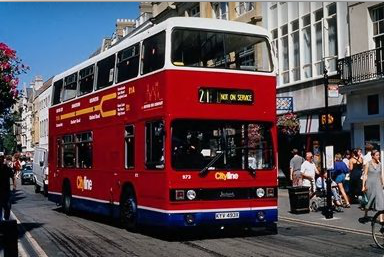
\includegraphics[scale=.4]{img/3005_chi.png}}


\caption{Town Scene. Using chi-square as similarity measure.}
\label{fig:5}
\end{figure}

\begin{figure}
\centering
\subfloat[][]{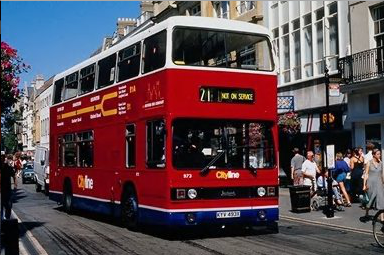
\includegraphics[scale=.4]{img/3001_bhat.png}}
\quad
\subfloat[][]{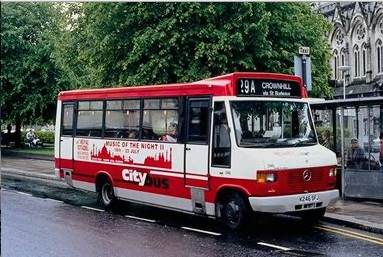
\includegraphics[scale=.4]{img/3002_bhat.png}}
\quad
\subfloat[][]{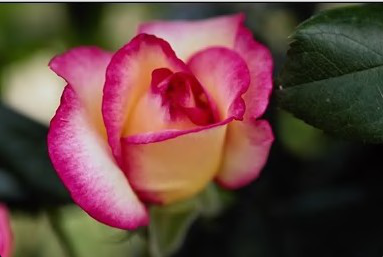
\includegraphics[scale=.4]{img/3003_bhat.png}}
\quad
\subfloat[][]{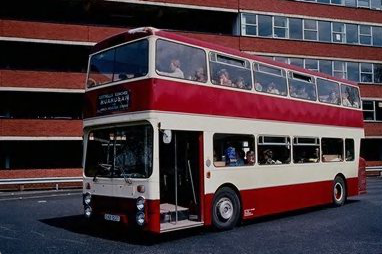
\includegraphics[scale=.4]{img/3004_bhat.png}}

\subfloat[][]{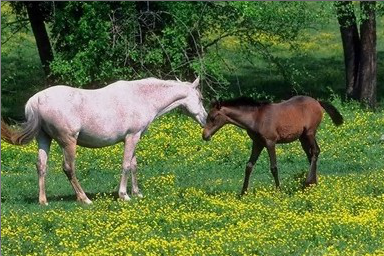
\includegraphics[scale=.4]{img/3005_bhat.png}}


\caption{Town Scene. Using Bhattacharyya distance as similarity measure.}
\label{fig:7}
\end{figure}

\begin{figure}
\centering
\subfloat[][]{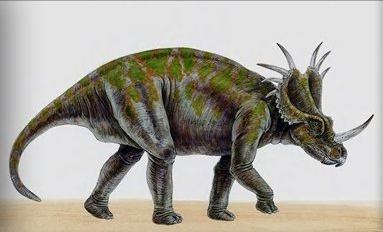
\includegraphics[scale=.4]{img/4001_corr.png}}
\quad
\subfloat[][]{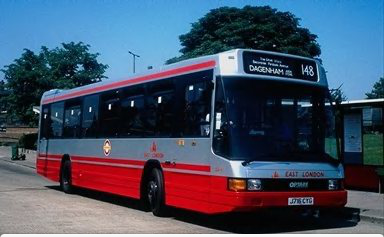
\includegraphics[scale=.4]{img/4002_corr.png}}
\quad
\subfloat[][]{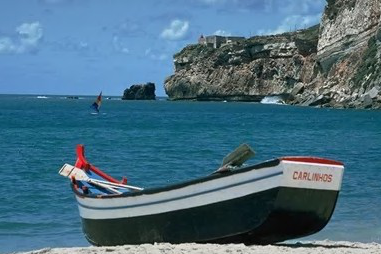
\includegraphics[scale=.4]{img/4003_corr.png}}
\quad
\subfloat[][]{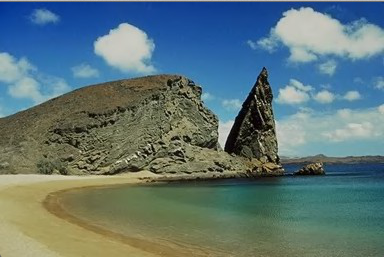
\includegraphics[scale=.4]{img/4004_corr.png}}

\subfloat[][]{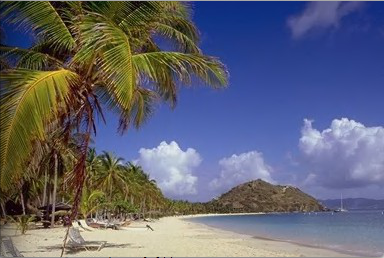
\includegraphics[scale=.4]{img/4005_corr.png}}


\caption{Dinosaurs. Using correlation as similarity measure, but on images with equalized histograms. Note that for comparison, equalized histograms were used, but the original images are displayed.}
\label{fig:1}
\end{figure}











\end{document}
